%!TEX TS-program = xelatex 
%!TEX TS-options = -output-driver="xdvipdfmx -q -E"
%!TEX encoding = UTF-8 Unicode
%
%  my_title
%
%  Created by my_name on date.
%  Copyright (c) year. All rights reserved.
%

\documentclass[12pt]{article} 

% Definitions
\newcommand\mykeywords{color, illusion} 
\newcommand\myauthor{Mark Eli Kallderon} 
\newcommand\mytitle{Color Illusion}
\newcommand\mybib{Philosophy.bib}

% Packages
\usepackage{geometry} \geometry{a4paper} 
\usepackage{url}
\usepackage{txfonts}
\usepackage{color}
\definecolor{gray}{rgb}{0.459,0.438,0.471}
% \usepackage{setspace}
% \doublespace % Uncomment for doublespacing if necessary
\usepackage{epigraph} % optional

% XeTeX
\usepackage[cm-default]{fontspec}
\usepackage{xltxtra,xunicode}
\defaultfontfeatures{Scale=MatchLowercase,Mapping=tex-text}
\setmainfont{Palatino}
\setsansfont{Gill Sans}
\setmonofont{Inconsolata}

% Section Formatting
\usepackage[]{titlesec}
\titleformat{\section}[hang]{\fontsize{14}{14}\scshape}{\S{\thesection}}{.5em}{}{}
\titleformat{\subsection}[hang]{\fontsize{12}{12}\scshape}{\S{\thesubsection}}{.5em}{}{}
\titleformat{\subsubsection}[hang]{\fontsize{12}{12}\scshape}{\S{\thesubsubsection}}{.5em}{}{}

% Headers and Footers
\usepackage{fancyhdr}
\pagestyle{fancy}
\pagenumbering{arabic}
\lhead{\thepage}
\chead{}
\rhead{\itshape{\nouppercase{\leftmark}}}

% TODO List
\usepackage{color}
\usepackage{index} % use index package to create indices
\newindex{todo}{tod}{tnd}{TODO List} % start todo list
\newindex{fixme}{fix}{fnd}{FIXME List} % start fixme list
\newcommand{\todo}[1]{\textcolor{blue}{TODO: #1}\index[todo]{#1}} % macro for todo entries
\newcommand{\fixme}[1]{\textcolor{red}{FIXME: #1}\index[fixme]{#1}} % macro for fixme entries

% Bibliography
\usepackage[round]{natbib} 

% Title Information
\title{\mytitle} % For thanks comment this line and uncomment the line below
%\title{\mytitle\thanks{}}% 
\author{\myauthor} 
% \date{} % Leave blank for no date, comment out for most recent date

% PDF Stuff
\usepackage[plainpages=false, pdfpagelabels, bookmarksnumbered, backref, pdftitle={\mytitle}, pagebackref, pdfauthor={\myauthor}, pdfkeywords={\mykeywords}, xetex, dvipdfmx, colorlinks=true, citecolor=gray, linkcolor=gray, urlcolor=gray]{hyperref} 



%%% BEGIN DOCUMENT
\begin{document}

% Title Page
\maketitle
% \begin{abstract} % optional
% \end{abstract} 
\vskip 2em \hrule height 0.4pt \vskip 2em
% \epigraph{text of epigraph}{\textsc{author of epigraph}} % optional; make sure to uncomment \usepackage{epigraph}

% Layout Settings
\setlength{\parindent}{1em}

% Main Content

\section{Introduction} % (fold)
\label{sec:introduction}

I have lost my grip on what a color illusion is meant to be. Perhaps I have simply lost my grip---not an alternative to be ruled out in advance of inquiry. However, I believe that there is an alternative explanation. I have come to suspect that there is nothing answering to the philosopher's conception of illusion. That's not to say that there are no color experiences that might, with propriety, be described as illusory. There is a familiar genre of books illustrating optical illusions, many essentially involving chromatic phenomena. No charge of false advertising is leveled here. It is only a distinctively philosophical conception of illusion whose claims are exaggerated. Or so I have, lately, come to suspect.

% section introduction (end)

\section{Benham's Disk} % (fold)
\label{sec:benham_s_disk}

Let's begin by considering an example of a color illusion often cited by philosophers, Benahma's disk.

In 1895, an English toymaker, Charles Benham, sold a top adorned with a black and white pattern (see Figure~\ref{fig:benham}).

\begin{figure}[htbp]
	\centering
		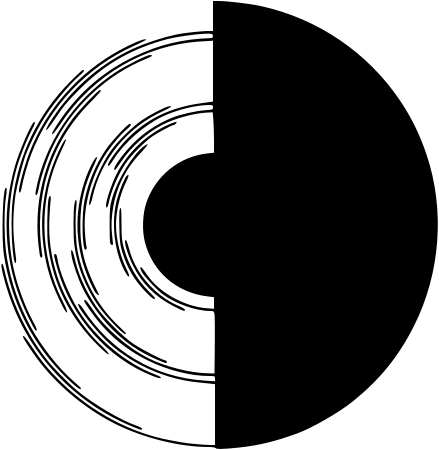
\includegraphics[scale=.5]{graphics/benhams_disk.jpg}
	\caption{Benham's Disk}
	\label{fig:benham}
\end{figure}



% section benham_s_disk (end)

% Bibligography
% \bibliographystyle{plainnat} 
% \bibliography{\mybib} 

\end{document}
